% \begin{document}
\section{Algorithm for Maximum Cardinality Bipartite Matching}
\subsection{Duality}

Before giving an algorithm, perhaps an easier question is: how would you give a short proof that
a given matching is optimal?

For this purpose, one would like to find upper bounds on the size of the largest matching and hope
that the smallest of these upper bounds be equal to the size of the largest matching. This is a
duality concept that will be very important in this subject. In this case, the dual problem will
be a famous combinatorial optimization problem: \emph{vertex cover}.

\paragraph{Vertex cover:} A vertex cover is a set $C$ of vertices so that all edges $e$ of $E$ are
incident to at least one edge in $C$. In other words, there is no edge completely contained in
$V\setminus C$.

We clearly have the following:
\[
  |M|\le|C| \quad\text{for any matching $M$ and vertex cover $C$.}
\]
This follows from the fact that, given any matching $M$, a vertex cover $C$ must contain at least
one of the end points of each edge in $M$.

This is \emph{weak duality}: The maximum size of a matching is at most the minimum size of a
vertex cover. We shall in fact prove \emph{strong duality} (that equality holds) for bipartite
graphs:

\label{thm:konig}
\thm{K\"onig 1931}{
For any bipartite graph, the maximum size of a matching is equal to the minimum size of a vertex
cover.
}

The proof of this theorem will be algorithmic. It will give an efficient algorithm for both
finding a maximum size matching and a minimum size vertex cover of a bipartite graph. Note that
whenever one has min max statement as above, the problem lies in $\mathsf{NP}\cap\mathsf{coNP}$
which may indicate that it has an efficient algorithm.

\label{ex:konig}
\ex{}{
The edges $(1,6),(2,7),(3,8)$ and $(5,10)$ form a matching (of maximum cardinality). Vertices
$1,2,5$, and $8$ form a vertex cover (of minimum cardinality).

\begin{center}
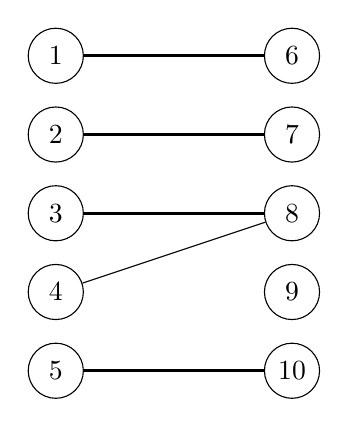
\begin{tikzpicture}[every node/.style={circle,draw,minimum size=7mm,inner sep=0pt}]
  \foreach \i in {1,...,5} {
    \node (\i) at (0,{5-\i}) {\i};
  }
  \foreach \i in {6,...,10} {
    \node (\i) at (3,{10-\i}) {\i};
  }
  \draw[very thick] (1) -- (6);
  \draw[very thick] (2) -- (7);
  \draw[very thick] (3) -- (8);
  \draw[very thick] (5) -- (10);
  \draw (4) -- (8);
\end{tikzpicture}
\end{center}
}

\subsection{Algorithm}

Recall that a path is a collection of edges $(v_0,v_1),(v_1,v_2),\ldots,(v_{k-1},v_k)$ where the
$v_i$'s are distinct vertices. We can simply represent a path as $v_0-v_1-v_2-\ldots-v_k$.

\dfn{Alternating path}{
An \emph{alternating path} with respect to $M$ is a path that alternates between edges in $M$ and
edges in $E\setminus M$.
}

\dfn{Augmenting path}{
An \emph{augmenting path} with respect to $M$ is an alternating path in which the first and last
vertices are unmatched.
}

\begin{figure}[h]
\centering
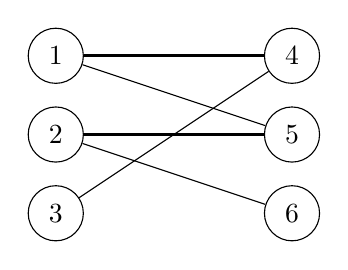
\begin{tikzpicture}[every node/.style={circle,draw,minimum size=7mm,inner sep=0pt}]
  \node (1) at (0,2) {1};
  \node (2) at (0,1) {2};
  \node (3) at (0,0) {3};
  \node (4) at (3,2) {4};
  \node (5) at (3,1) {5};
  \node (6) at (3,0) {6};
  \draw (3) -- (4);
  \draw[very thick] (4) -- (1);
  \draw (1) -- (5);
  \draw[very thick] (5) -- (2);
  \draw (2) -- (6);
\end{tikzpicture}
\caption{The edges $(3,4),(4,1),(1,5),(5,2),(2,6)$ form an augmenting path}
\end{figure}

The definition of an augmenting path motivates the following algorithm:

\bigskip
\noindent\fbox{\parbox{0.95\textwidth}{
\textbf{\AugAlg$(G)$:}\\[2pt]
\textbf{Input:} A bipartite graph $G=(V,E)$.\\
\textbf{Output:} A matching $M$ of maximum cardinality.
\begin{enumerate}[leftmargin=2em,label=\arabic*.]
  \item Initialize $M=\emptyset$.
  \item \textbf{while} exists an augmenting path $P$
  \item \hspace{1em}update $M=M\Delta P\equiv (M\setminus P)\cup(P\setminus M)$.
  \item \textbf{return} $M$.
\end{enumerate}
}}
\bigskip

\ex{Exercise}{
Devise an efficient algorithm for finding an augmenting path $P$ (if one exists). What is the
total running time of the \AugAlg{}?
}

We now prove that \AugAlg{} indeed finds a maximum matching.

\label{thm:aug}
\thm{}{
A matching $M$ is maximum if and only if there are no augmenting paths with respect to $M$.
}

\pf{}{
($\Rightarrow$) Let $P$ be some augmenting path with respect to $M$. Then $M'=M\Delta P$ is
matching of greater cardinality than $M$. This contradicts the optimality of $M$.

($\Leftarrow$) If $M$ is not maximum, let $M^*$ be a maximum matching so that $|M^*|>|M|$. Let
$Q=M\Delta M^*$. Then
\begin{itemize}
  \item $Q$ has more edges from $M^*$ than from $M$ (since $|M^*|>|M|$ implies that
    $|M^*\setminus M|>|M\setminus M^*|$).
  \item Each vertex is incident to at most one edge in $M\cap Q$ and one edge in $M^*\cap Q$.
  \item Thus $Q$ is composed of cycles and paths that alternate between edges from $M$ and $M^*$.
  \item Therefore there must be some path with more edges from $M^*$ in it than from $M$. This
    path is an augmenting path with respect to $M$.
\end{itemize}
Hence, there must exist an augmenting path $P$ with respect to $M$, which is a contradiction.
}

\subsection{Proof of K\"onig's Theorem}

Consider a maximum matching $M^*$ of $G=(A\cup B,E)$. Let $L$ the vertices reachable from
unmatched vertices in $A$ by alternating paths with respect to $M^*$. (So e.g.\ in the figure of
Example~\ref{ex:konig} $L=\{4,8,3\}$.) The following proves K\"onig's theorem.
\label{lem:cover}
\mlenma{}{
We have that $C^*=(A\setminus L)\cup(B\cap L)$ is a vertex cover. Moreover, $|C^*|=|M^*|$.
}

\pf{}{
We first show that $C^*$ is a vertex cover. Suppose toward contradiction that it is not. Then
there is an edge $e=(a,b)\in E$ with $a\in A\cap L$ and $b\in B\setminus L$. The edge cannot
belong to the matching. If it did then $b$ should be in $L$ because otherwise $a$ would not be in
$L$. Hence $e\in E\setminus M$. This however, implies that there is an alternating path from an
unmatched vertex to $b$ (namely go to $a$ and take the edge $(a,b)$) contradicting the fact that
$b\notin L$.

To show the second part of the proof, we show that $|C^*|\le|M^*|$, since the reverse inequality
is true for any matching and any vertex cover. The proof follows from the following observations:
\begin{enumerate}
  \item No vertex in $A\setminus L$ is unmatched by the definition of $L$;
  \item No vertex in $B\cap L$ is unmatched since this would imply the existence of an augmenting
    path (which contradicts that $M^*$ is optimal).
  \item There is no edge of the matching between a vertex $a\in A\setminus L$ and a vertex
    $b\in B\cap L$. Otherwise $a$ would be in $L$.
\end{enumerate}
These remarks imply that every vertex in $C^*$ is matched and moreover the corresponding edges of
the matching are distinct. Hence, $|C^*|\le|M^*|$.
}

% \end{document}
